\documentclass[10pt,winfonts,fancyhdr,hyperref,UTF8]{ctexrep}
\usepackage{indentfirst} 
\usepackage{fontspec}
\usepackage{titlesec}
\usepackage{xeCJK}
\usepackage{graphicx}
\usepackage{ifthen}
\usepackage{color,fancyvrb}
\usepackage{listings}
\usepackage{syntonly}
\usepackage{makeidx}
\usepackage[hidelinks, colorlinks=true]{hyperref}
\usepackage{algorithm}
\usepackage{algpseudocode}
\usepackage{amssymb}
\usepackage{multirow}
\usepackage{ulem}
\usepackage{diagbox}
\makeatletter
%LeetCode Setting
\usepackage[centering,paperwidth=180mm,paperheight=230mm,%
body={390pt,530pt},marginparsep=10pt,marginpar=50pt]{geometry}
\usepackage{color}
\usepackage{enumitem}
\usepackage{fancyvrb}
\usepackage[bottom,perpage,symbol*]{footmisc}
\usepackage{graphicx}
\usepackage[hidelinks]{hyperref}
\usepackage{makeidx}
\usepackage[toc]{multitoc}
\usepackage{pifont}
\usepackage{underscore}
\usepackage{amsmath}

\DefineFNsymbols*{chinese}{{\ding{172}}{\ding{173}}{\ding{174}}{\ding{175}}%
{\ding{176}}{\ding{177}}{\ding{178}}{\ding{179}}{\ding{180}}{\ding{181}}}
\setfnsymbol{chinese}

\hypersetup{bookmarksnumbered=true,bookmarksdepth=2}

\CTEXsetup[number={\thechapter}]{chapter}
\CTEXsetup[format+={\raggedleft}]{chapter}
\CTEXsetup[beforeskip={10pt}]{chapter}
\CTEXsetup[afterskip={30pt}]{chapter}
\def\CTEX@chapter@aftername{\par} % \CTEXsetup[aftername={\par}]{chapter}
\CTEXsetup[format+={\raggedright}]{section}
\CTEXsetup[beforeskip={-3.0ex plus -1ex minus -.2ex}]{section}
\CTEXsetup[afterskip={2.3ex plus .2ex minus 0.2ex}]{section}

\renewcommand \thefigure{\thechapter-\arabic{figure}}
\renewcommand \thetable{\thechapter-\arabic{table}}

\newcommand\figcaption[1]{\def\@captype{figure}\caption{#1}}
\newcommand\tabcaption[1]{\def\@captype{table}\caption{#1}}

\long\def\@caption#1[#2]#3{%
  \addcontentsline{\csname ext@#1\endcsname}{#1}%
    {\protect\numberline{\csname fnum@#1\endcsname}{ \ignorespaces #2}}% change "the" to "fnum@"
    \normalsize
    \@makecaption{\csname fnum@#1\endcsname}{\ignorespaces #3}}

\long\def\@makecaption#1#2{%
  \vskip\abovecaptionskip
  \sbox\@tempboxa{#1\quad#2}%
  \ifdim \wd\@tempboxa >\hsize
    #1\quad#2\par
  \else
    \global \@minipagefalse
    \hb@xt@\hsize{\hfil\box\@tempboxa\hfil}%
  \fi
  \vskip\belowcaptionskip}

\setlength\abovecaptionskip{0pt}
  
\setmainfont{Times New Roman}
%\setmainfont{Linux Libertine}
%\setmainfont{TeX Gyre Pagella}
\newfontfamily\urlfont{Times New Roman}
%\setmonofont[AutoFakeBold=1.6,AutoFakeSlant=0.17,Mapping=tex-text-tt]{Inconsolata}
\setCJKfamilyfont{zhyou}{YouYuan}

\newcommand{\fn}[1]{\texttt{#1}}
\newcommand{\sfn}[1]{\texttt{\small #1}}
\newcommand{\kw}[1]{\textsf{#1}}
\newcommand{\myurl}[1]{{\urlfont #1}}
\newcommand{\mpar}[1]{\marginpar[\hfill\kaishu #1]{\kaishu #1}}
\newcommand{\mn}[1]{\texttt{\bs #1}}
\renewcommand{\today}{\the\year-\the\month-\the\day}
\newcommand\bs{\textbackslash}
\newcommand{\code}[1]{\small{\fontspec{Latin Modern Mono} #1}}

\newcommand\begindot{\begin{itemize}
[itemsep=2pt plus 2pt minus 2pt,%
topsep=3pt plus 2pt minus 2pt,%
parsep=0pt plus 2pt minus 2pt]}
\newcommand\myenddot{\end{itemize}}

\newcommand\beginnum{\begin{enumerate}
[itemsep=2pt plus 2pt minus 2pt,%
topsep=3pt plus 2pt minus 2pt,%
parsep=0pt plus 2pt minus 2pt]}
\newcommand\myendnum{\end{enumerate}}

\DefineVerbatimEnvironment%
  {Code}{Verbatim}
  {fontsize=\small,baselinestretch=0.9,xleftmargin=3mm}

\raggedbottom
%\setlength{\parskip}{1ex plus .5ex minus .5ex}

\def\FV@SetLineWidth{%
  \if@FV@ResetMargins\else
    \advance\leftmargin\@totalleftmargin
  \fi
  \advance\leftmargin\FV@XLeftMargin\relax
  \advance\rightmargin\FV@XRightMargin\relax
  \linewidth\hsize
  %\advance\linewidth-\leftmargin
  %\advance\linewidth-\rightmargin
  \hfuzz\FancyVerbHFuzz\relax}


\def\FV@SingleFrameLine#1{%
%% DG/SR modification end
  \hbox to\z@{%
    %\kern\leftmargin
%% DG/SR modification begin - Jun. 22, 1998
    \ifnum#1=\z@
      \let\FV@Label\FV@LabelBegin
    \else
      \let\FV@Label\FV@LabelEnd
    \fi
    \ifx\FV@Label\relax
%% DG/SR modification end
      \FancyVerbRuleColor{\vrule \@width\linewidth \@height\FV@FrameRule}%
%% DG/SR modification begin - Jun. 22, 1998
    \else
      \ifnum#1=\z@
        \setbox\z@\hbox{\strut\enspace\urlfont\FV@LabelBegin\strut}%
      \else
        \setbox\z@\hbox{\strut\enspace\urlfont\FV@LabelEnd\strut}%
      \fi
      \@tempdimb=\dp\z@
      \advance\@tempdimb -.5\ht\z@
      \@tempdimc=\linewidth
      \advance\@tempdimc -\wd\z@
      %\divide\@tempdimc\tw@
      \ifnum#1=\z@              % Top line
        \ifx\FV@LabelPositionTopLine\relax
          \FancyVerbRuleColor{\vrule \@width\linewidth \@height\FV@FrameRule}%
        \else
          \FV@FrameLineWithLabel
        \fi
      \else                     % Bottom line
        \ifx\FV@LabelPositionBottomLine\relax
          \FancyVerbRuleColor{\vrule \@width\linewidth \@height\FV@FrameRule}%
        \else
          \FV@FrameLineWithLabel
        \fi
      \fi
    \fi
%% DG/SR modification end
    \hss}}


%% DG/SR modification begin - May. 19, 1998
\def\FV@FrameLineWithLabel{%
  \ht\z@\@tempdimb\dp\z@\@tempdimb%
  \FancyVerbRuleColor{%
    \raise 0.5ex\hbox{\vrule \@width\@tempdimc \@height\FV@FrameRule}%
    \raise\@tempdimb\box\z@}}
%% DG/SR modification end


\def\FV@EndListFrame@Lines{%
  \begingroup
    %\vskip 0.5ex
    \baselineskip\z@skip
    \kern\FV@FrameSep\relax
%% DG/SR modification begin - May. 19, 1998
%%    \FV@SingleFrameLine
    \FV@SingleFrameLine{\@ne}%
%% DG/SR modification end
  \endgroup}

\newskip\mytopsep
\setlength{\mytopsep}{4pt plus 2pt minus 3pt}

\def\FV@ListVSpace{%
  \@topsepadd\mytopsep
  \if@noparlist\advance\@topsepadd\partopsep\fi
  \if@inlabel
    \vskip\parskip
  \else
    \if@nobreak
      \vskip\parskip
      \clubpenalty\@M
    \else
      \addpenalty\@beginparpenalty
      \@topsep\@topsepadd
      \advance\@topsep\parskip
      \addvspace\@topsep
    \fi
  \fi
  %\showthe \@topsepadd
  %\showthe \topsep
  %\showthe \partopsep
  %\showthe \parskip
  \global\@nobreakfalse
  \global\@inlabelfalse
  \global\@minipagefalse
  \global\@newlistfalse}

\def\FV@EndList{%
  \FV@ListProcessLastLine
  \FV@EndListFrame
  %\showthe \@topsepadd
  \@endparenv
  \endgroup
  \@endpetrue}

\def\theFancyVerbLine{\sffamily\scriptsize\arabic{FancyVerbLine}}

\DefineVerbatimEnvironment%
  {Codex}{Verbatim}
  {fontsize=\small,baselinestretch=0.9,xleftmargin=3mm,%
  frame=lines,labelposition=all,framesep=5pt}

\DefineVerbatimEnvironment%
  {Code}{Verbatim}
  {fontsize=\small,baselinestretch=0.9,xleftmargin=3mm}

\makeindex

%Other settings:
\lstset{%  
  alsolanguage=Java,  
  language={C++},
  tabsize=4, %  
  frame=shadowbox, %把代码用带有阴影的框圈起来  
  commentstyle=\color{red!50!green!50!blue!50},%浅灰色的注释  
  rulesepcolor=\color{red!20!green!20!blue!20},%代码块边框为淡青色  
  keywordstyle=\color{blue!90}\bfseries, %代码关键字的颜色为蓝色,粗体  
  showstringspaces=false,%不显示代码字符串中间的空格标记  
  stringstyle=\ttfamily, % 代码字符串的特殊格式  
  keepspaces=true, %  
  breakindent=22pt, %  
  numbers=left,%左侧显示行号 往左靠,还可以为right,或none,即不加行号  
  stepnumber=1,%若设置为2,则显示行号为1,3,5,即stepnumber为公差,默认stepnumber=1  
  %numberstyle=\tiny, %行号字体用小号  
  numberstyle={\color[RGB]{0,192,192}\tiny} ,%设置行号的大小,大小有tiny,scriptsize,footnotesize,small,normalsize,large等  
  numbersep=8pt,  %设置行号与代码的距离,默认是5pt  
  basicstyle=\footnotesize, % 这句设置代码的大小  
  showspaces=false, %  
  flexiblecolumns=true, %  
  breaklines=true, %对过长的代码自动换行  
  breakautoindent=true,%  
  breakindent=4em, %  
  aboveskip=1em, %代码块边框  
  tabsize=2,  
  showstringspaces=false, %不显示字符串中的空格  
  backgroundcolor=\color[RGB]{245,245,244},   %代码背景色  
}















\makeatother
%\graphicspath{{images/}}

\usepackage{tikz}
\usetikzlibrary{calc}
\usetikzlibrary{fit}
\usetikzlibrary{positioning}
\usepgflibrary{plotmarks}

\usetikzlibrary{shapes.geometric}

\CustomVerbatimEnvironment{shellcmd}{Verbatim}
{frame=single,rulecolor=\color{blue},framerule=3pt,framesep=1pc,fillcolor=\color{yellow}}

\newcommand{\bookname}{TechNotes}
\renewcommand{\contentsname}{Algorithms} 

\title{\sffamily Algorithms}
\date{\today}
\setcounter{tocdepth}{1}
\setcounter{chapter}{0}

\begin{document}

%\maketitle
\tableofcontents


%TOADD
%!Mode:: "TeX:UTF-8"
\chapter{算法}

%!Mode:: "TeX:UTF-8"
\section{B树及其变体}

\subsection{B树}
B树(B-tree)是一种树状数据结构,它能够存储数据、对其进行排序并允许以O(log n)的时间复杂度运行进行查找、顺序读取、插入和删除的数据结构。B树,概括来说是一个节点可以拥有多于2个子节点的二叉查找树。与自平衡二叉查找树不同,B树为系统最优化大块数据的读和写操作。B-tree算法减少定位记录时所经历的中间过程,从而加快存取速度。普遍运用在数据库和文件系统。

\begin{figure}[ht]
	\begin{center}
		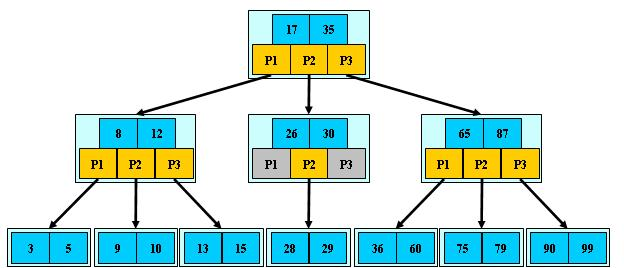
\includegraphics[keepaspectratio,width=0.6\paperwidth]{Pictures/BTree/BTreeBlogPicture.jpg}
	\caption{B树}
	\label{fig:BTreeBlogPicture}
	\end{center}
\end{figure}


根据Knuth的定义,m阶B树符合下列条件:
\begin{enumerate}
  \item 每个结点至多有m个子结点
  \item 除根结点外,非叶结点至少有$\lceil m/2 \rceil$ 个子结点
  \item 根结点至少有两个子结点,除非它是叶结点
  \item 非叶结点的关键词树比其子结点树少1
  \item 叶结点在同一层
\end{enumerate}
树的高度$h$(如果根结点为叶节点,高度为0)满足:$h \le \log_{\lceil m/2 \rceil}(\frac{n+1}{2})$。其中$n$为关键词数。

\subsection{B树操作}

\subsubsection{B树的搜索search(root, target)}
从root出发,对每个节点,找到大于或等于target关键字中最小的K[i],如果K[i]与target相等,则查找成功;否则在P[i]中递归搜索target,直到到达叶子节点,如仍未找到则说明关键字不在B树中,查找失败。
 
\subsubsection{B树的插入,insert(root, target)}
B树的插入需要沿着搜索的路径从root一直到叶节点,根据B树的规则,每个节点的关键字个数在[t-1, 2t-1]之间,故当target要加入到某个叶子时,如果该叶子节点已经有2t-1个关键字,则再加入target就违反了B树的定义,这时就需要对该叶子节点进行分裂,将叶子以中间节点为界,分成两个包含t-1个关键字的子节点,同时把中间节点提升到该叶子的父节点中,如果这样使得父节点的关键字个数超过2t-1,则要继续向上分裂,直到根节点,根节点的分裂会使得树加高一层。
 
上面的过程需要回溯,那么能否从根下降到叶节点后不回溯就能完成节点的插入呢?答案是肯定的,核心思想就是未雨绸缪,在下降的过程中,一旦遇到已满的节点(关键字个数为2t-1),就就对该节点进行分裂,这样就保证在叶子节点需要分裂时,其父节点一定是非满的,从而不需要再向上回溯。
 
\subsubsection{B树的删除,delete(root, target)}
在删除B树节点时,为了避免回溯,当遇到需要合并的节点时就立即执行合并,B树的删除算法如下:从root向叶子节点按照search规律遍历:
\begin{enumerate}
\item 如果target在叶节点x中,则直接从x中删除target,
情况(2)和(3)会保证当再叶子节点找到target时,肯定能借节点或合并成功而不会引起父节点的关键字个数少于t-1。
\item  如果target在分支节点x中:
	\begin{enumerate}
		\item 如果x的左分支节点y至少包含t个关键字,则找出y的最右的关键字prev,并替换target,并在y中递归删除prev。
		\item 如果x的右分支节点z至少包含t个关键字,则找出z的最左的关键字next,并替换target,并在z中递归删除next。
		\item 否则,如果y和z都只有t-1个关键字,则将targe与z合并到y中,使得y有2t-1个关键字,再从y中递归删除target。
	\end{enumerate}
\item 如果关键字不在分支节点x中,则必然在x的某个分支节点p[i]中,如果p[i]节点只有t-1个关键字:
	\begin{enumerate}
		\item 如果p[i-1]拥有至少t个关键字,则将x的某个关键字降至p[i]中,将p[i-1]的最大节点上升至x中。
		\item 如果p[i+1]拥有至少t个关键字,则将x个某个关键字降至p[i]中,将p[i+1]的最小关键字上升至x个。
		\item 如果p[i-1]与p[i+1]都拥有t-1个关键字,则将p[i]与其中一个兄弟合并,将x的一个关键字降至合并的节点中,成为中间关键字。
	\end{enumerate}
\end{enumerate}

\subsection{B+树和B*树数}
B+树是B树的变体,也是一种多路搜索树,其定义基本与B树同,除了:
\begin{enumerate}
  \item 非叶子结点的子树指针与关键字个数相同
  \item 非叶子结点的子树指针P[i],指向关键字值属于[K[i], K[i+1])的子树(B-树是开区间)
  \item 所有关键字都在叶子结点出现, 所有叶子结点增加一个链指针
\end{enumerate}
 B+的搜索与B-树也基本相同,区别是B+树只有达到叶子结点才命中(B-树可以在
非叶子结点命中),其性能也等价于在关键字全集做一次二分查找。

\begin{figure}[ht]
	\begin{center}
		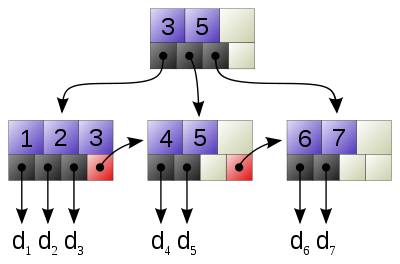
\includegraphics[keepaspectratio,width=0.6\paperwidth]{Pictures/BTree/BplusTree-wiki.png}
	\caption{B+树-维基百科图片}
	\label{fig:BplusTree-wiki}
	\end{center}
\end{figure}

B+树的特性:
\begin{enumerate}
  \item 所有关键字都出现在叶子结点的链表中(稠密索引),且链表中的关键字恰好是有序的
  \item 不可能在非叶子结点命中
  \item 非叶子结点相当于是叶子结点的索引(稀疏索引),叶子结点相当于是存储(关键字)数据的数据层
  \item 更适合文件索引系统
\end{enumerate}

\begin{figure}[ht]
	\begin{center}
		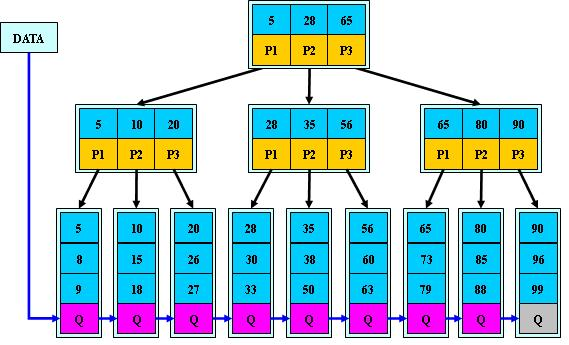
\includegraphics[keepaspectratio,width=0.6\paperwidth]{Pictures/BTree/BPlusTree.jpg}
	\caption{B+树}
	\label{fig:BplusTree}
	\end{center}
\end{figure}

Windows 文件系统NTFS 在 FAT 和 HPFS(高性能文件系统)的基础上作了一系列改进(如支持元数据)并且使用了更复杂的数据结构(B+树)以便于提升性能、改善可靠性并降低磁盘空间利用率。

B*树是B+树的变体,在B+树的非根和非叶子结点再增加指向兄弟的指针。
B*树定义了非叶子结点关键字个数至少为(2/3)*M,即块的最低使用率为2/3(代替B+树的1/2)。

B+树的分裂:当一个结点满时,分配一个新的结点,并将原结点中1/2的数据复制到新结点,最后在父结点中增加新结点的指针;B+树的分裂只影响原结点和父结点,而不会影响兄弟结点,所以它不需要指向兄弟的指针;

B*树的分裂:当一个结点满时,如果它的下一个兄弟结点未满,那么将一部分数据移到兄弟结点中,再在原结点插入关键字,最后修改父结点中兄弟结点的关键字(因为兄弟结点的关键字范围改变了);如果兄弟也满了,则在原结点与兄弟结点之间增加新结点,并各复制1/3的数据到新结点,最后在父结点增加新结点的指针;所以,B*树分配新结点的概率比B+树要低,空间使用率更高。

\clearpage










%!Mode:: "TeX:UTF-8"
\section{缓存替换算法}
LFRU,2Q。



%!Mode:: "TeX:UTF-8"
\section{二分查找代码示例}

注意事项:除以2的操作可改为右移操作。

程序可以有多种写法,主要有如下区别:
\begin{itemize}
    \item 不变式区间的开闭性。不变式:待搜数据t不存在,或属于不变式区间。区间可以为[l,u]或(l,u]。区间的开闭性影响迭代更新的方式。
    \item 每次循环的比较操作次数,可以为1次或两次。每次循环如果作两次判断,效率较低,但循环次数可能会减少,因为可以直接发现目标退出循环。可以将等于比较合并到大于或小于比较中来减少判断。
\end{itemize}


当区间长度至少为3时,下轮迭代区间必能能够缩小。当区间长度为2或1时,按照\verb|m=(u+l)/2|计算到的中点m即为左端点l,如果区间端点按照l=m方式来更新,会导致区间不能缩小。当区间长度为1时,m同时等于l和u,当区间右端点按照u=m来更新时,也会发生区间不能缩小的情形,如编程不慎则会造成死循环。

如果采用全闭区间-两次比较的方式编程,u和l都不会直接赋为m,则只需确保区间长度大于零即可,无死循环之虞。如果区间存在开端,或者只进行一次比较,则需要慎重。

可以对算法提出额外要求,即当存在多个满足条件的值时,应能返回下标最低者。

如果数组长度为固定值,如1000,可以通过循环展开以进一步优化代码。
虽然二分搜索可以在log时间内完成搜索,但搜索后如果要插入新元素仍需要线性时间。不过,基于数组的连续操作具有很好的cache友好性。

\subsection{半闭区间,单次比较}
\cite{pp}9.3。 x[-1],x[n]作哨兵,但未真正访问。u和l都会直接赋为m,因此循环条件是区间长度至少为3,即l+1 != u。t包含于(l,u]。左边为开,能够保证返回最低下标。
\label{codes:binsort}

\begin{lstlisting}[language=C]

int binarysearch3(DataType t)
{	
	int l = -1, u = n, m;
	while (l+1 != u) {
		m = (l + u) >> 1;
		if (x[m] < t) l = m;
		else u = m;
	}
	if (u >= n || x[u] != t) return -1;
	return u;
}
\end{lstlisting}

然而,我并未发现为何将u初始化为n,而不是n-1。我认为初始化为n-1更简洁,相应代码为:
\begin{lstlisting}[language=Python]

#!/usr/bin/env python

"""
binary sort implementation
"""

def BinSort(x, t):
    l = -1
    u = len(x) - 1
    while u - l >= 2:
        m = l + (u - l) / 2;
        if x[m] < t:
            l = m
        else:
            u = m
    
    if x[u] == t:
        return u
    else: 
        return -1



if __name__ == '__main__':

    assert BinSort([2], 3) == -1
    assert BinSort([2], 2) == 0
    assert BinSort([2], 1) == -1
    assert BinSort([2, 3], 1) == -1
    assert BinSort([2, 3], 4) == -1
    assert BinSort([2, 3], 2) == 0
    assert BinSort([2, 3], 3) == 1
    assert BinSort([2, 3, 4], 3) == 1
    assert BinSort([2, 3, 4], 2) == 0
    assert BinSort([2, 3, 4], 4) == 2
    assert BinSort([2, 3, 4], 5) == -1
    assert BinSort([2, 3, 4], 1) == -1
    assert BinSort([2, 3, 4], 2.5) == -1
    assert BinSort([2, 3, 4], 3.5) == -1
    assert BinSort([2, 3, 4, 5], 3.5) == -1
    assert BinSort([2, 3, 4, 5], 4.5) == -1
    assert BinSort([2, 3, 4, 5], 4) == 2
    assert BinSort([2, 3, 4, 5], 0) == -1

\end{lstlisting}

\subsection{半闭区间双次比较}
将单次比较改为双次比较没有难度。只需要多加一次相等比较。

\begin{lstlisting}[language=C]

int binarysearch3(DataType t)
{	
	int l = -1, u = n, m;
	while (l+1 != u) {
		m = (l + u) / 2;
		if (x[m] < t) l = m;
		else if x[m] &=& t return m;
		else u = m;
	}
	if (u >= n || x[u] != t) return -1;
	return u;
}
\end{lstlisting}

\subsection{闭区间单比较}
\cite{self}一段Python代码:
\begin{lstlisting}[language=Python]

def binsearch(x, n, t):
    #range size >= 1
    assert n > 0

    if x[0] > t or x[n-1] < t: return -1;

    l = 0
    u = n-1
    while (u-l >= 1): 
        #x[l] <= t <= x[u], l == 0 or x[l-1] < t, range size >= 2
        m = l + (u - l) / 2;
        print "[%d - %d], %d"%(l,u,m)
        if x[m] < t: 
            l = m + 1
        else: 
            u = m
    
    #range size is 1 
    if x[l] == t: return l
    return -1

\end{lstlisting}

\cite{bop}3.11也给出了闭区间单次比较算法的实现,该实现不满足返回最小下标的条件。代码没有对输入参数进行检查,如果输入区间为零,程序功能可能与期望不符。书中认为求midIndex不可以相加除以2,以防溢出。其实如此大数本不太可能作为数组的长度。
因为l按照来l=m方式更新,所以区间长度为2时即需要退出循环。更新u的方式也过于保守,是按照开区间的方式进行更新。

其代码的Python等效版本写为:
\begin{lstlisting}[language=Python]

def binsearch(x,l,u,t):
    while (l < u - 1): #range lengh >= 3 
        m = l + (u - l) / 2;
        print "[%d - %d], %d"%(l,u,m)
        if x[m] <= t:
            l = m
        else: 
            u = m # better be u = m-1
    
    #range size is 2 or 1 
    if x[u] == t: return u
    if x[l] == t: return l
    return -1

\end{lstlisting}

原书程序为:

\begin{lstlisting}[language=C]
int bisearch(char** arr, int b, int e, char* v)
{
    int minIndex = b, maxIndex = e, midIndex;
    //循环结束有两种情况:
    //若minIndex为偶数则minIndex ==  maxIndex
    //否则就是minIndex ==  maxIndex -1
    while (minIndex < maxIndex -1)
    {
	minIndex = minIndex + (maxIndex - minIndex) / 2;
	if (strcmp(arr[minIndex], v) <= 0)
	{
	    minIndex = midIndex;
	}
	else
	{
	    //不需要minIndex - 1, 防止minIndex == maxIndex
	    maxIndex = midIndex;
	}
    }

    if (!strcmp(arr[maxIndex],v))//先判断序号最大的值
    {
	return maxIndex;
    }
    else if (!strcmp(arr[minIndex],v))
    {
	return minIndex;
    }
    else
    {
	return -1;
    }
}
\end{lstlisting}


\subsection{闭区间双次比较}
\cite{pp}5.1。t包含于[l,u]。u和l都不会赋值为m。循环条件是区间长度至少为1,即l<=u。退出循环则意味着无解。如果一开始元素个数就为零,自然无法进入循环,算作无解。
\begin{lstlisting}[language=C]
int binarysearch2(DataType t)
{	
	int l, u, m;
	l = 0;
	u = n-1;
	while (l <= u) //区间大于等于1 
	{
		m = (l + u) / 2;
		if (x[m] < t)
			l = m+1;
		else if (x[m] == t)
			return m;
		else /* x[m] > t */
			u = m-1;
	}

	return -1;
}


\end{lstlisting}

\cite{sedgewick}P99也给出了这种算法:

\begin{lstlisting}[language=Java]
private int rank(int key)
{ // Binary search.
    int lo = 0;
    int hi = a.length - 1;
    while (lo <= hi)
    { // Key is in a[lo..hi] or not present.
	int mid = lo + (hi - lo) / 2;
	if (key < a[mid]) hi = mid - 1;
	else if (key > a[mid]) lo = mid + 1;
	else
	return mid;
    }
    return -1;
}

\end{lstlisting}









%!Mode:: "TeX:UTF-8"

\section{代码:二叉树非递归遍历}

\begin{lstlisting}[language=C++]

#include <iostream>
#include <stack>
using namespace std;

struct Node {
    Node *left;
    Node *right;
    int data;
    Node(Node *l, Node *r, int d = 0) :left(l), right(r), data(d) { }
    void visit() {
        cout << data << endl;
    }
};

enum TreeTraverseWay {
    TREE_PRE_ORDER,
    TREE_MID_ORDER,
    TREE_POST_ORDER,
};

void TreeTraverse(Node *tree, int way)
{
    if (!tree) return;
    stack<Node*> s;
    Node sentinel(0, 0);
    s.push(&sentinel);//sentinel

    Node *pre = &sentinel;
    Node *cur = tree;

    //invariant: stack top is cur's parent, parent on top of a child
    while (cur != &sentinel) 
    {
        if (pre != cur->left && pre != cur->right) //top -> down
        {
            if (cur->left) {
                if (TREE_PRE_ORDER == way) cur->visit();
                s.push(cur);
                pre = cur;
                cur = cur->left;
            } else if (cur->right) {
                if (TREE_MID_ORDER == way) cur->visit();
                s.push(cur);
                pre = cur;
                cur = cur->right;
            } else {//cur is leaf
                cur->visit();
                pre = cur;
                cur = s.top();
                s.pop();
            }
        } 
        else //down -> top
        { 
            if (pre == cur->left && cur->right) {
                if (TREE_MID_ORDER == way) cur->visit();
                s.push(cur);
                pre = cur;
                cur = cur->right;
            } else { //no more children
                if (TREE_POST_ORDER == way) cur->visit();
                pre = cur;
                cur = s.top();
                s.pop();
            }
        }
    }
}

int main ()
{
    const int maxnode = 1<<4;
    Node *node[maxnode];
    for (int i = maxnode-1; i > 0; i--)
    {
        node[i] = new Node((i>=(maxnode>>1)?0:node[2*i]), (i>=(maxnode>>1)?0:node[2*i+1]), i);
    }

    Node *root = node[1];
    node[3]->left = 0;

    //TreeTraverse(root, TREE_PRE_ORDER);
    //TreeTraverse(root, TREE_POST_ORDER);
    TreeTraverse(root, TREE_MID_ORDER);

    for (int i = maxnode-1; i > 0; i--)
    {
        delete node[i];
    }

    return 0;
}

\end{lstlisting}

%!Mode:: "TeX:UTF-8"
\section{图相关算法}
图有邻接表和邻接矩阵两种表示方式。对于稠密图,$E=\Theta(|V|^2)$。

广度优先搜索(BFS)伪代码:
\begin{lstlisting}[language=bash]
BFS(G, s)
  for u ← V[G] - {s}
       do color[u] ← WHITE
          d[u] ← INFINITY
          p[u] ← NIL
  color[s] ← GRAY
  d[s] ← 0
  p[s] ← NIL
  Q ← Ø
  ENQUEUE(Q, s)
  while Q != Ø
      do u ← DEQUEUE(Q)
         for v ← Adj[u] 
             do if color[v] = WHITE
                   then color[v] ← GRAY
                        d[v] ← d[u] + 1
                        p[v] ← u
                        ENQUEUE(Q, v)
         color[u] ← BLACK
\end{lstlisting}
由于每个顶点出队、入队各一次,扫描邻接表时每个边被扫描一次(聚集分析),因此BFS的运行时间为$O(V+E)$。

%DFS是对前序遍历的推广。
%如果G是一棵树,由于$|E|=\Theta(|V|)$,那么该树的所有顶点在总时间$|E|$都能被访问到。
深度优先搜索(DFS)伪代码:
\begin{lstlisting}[language=bash]
DFS(G)
  for u ← V[G]
       do color[u] ← WHITE
          p[u] ← NIL
  time ← 0
  for u ← V[G]
       do if color[u] = WHITE
             then DFS-VISIT(u)

DFS-VISIT(u)
  color[u] ← GRAY
  d[u] ← ++time
  for v ← Adj[u] 
       do if color[v] = WHITE
             then p[v] ← u
                 DFS-VISIT(v)
  color[u] ← BLACK
  f[u] ← ++time
\end{lstlisting}
每个结点调用DFS-VISIT一次。利用聚集分析可知,DFS的运行时间为$O(V+E)$。

\subsection{单源最短路径}
对于路径无权值情形,使用广度优先搜索即可。

如果路径有\textbf{非负}权值,可使用Dijkstra算法。Dijkstra算法是贪心算法的很好的例子。




\begin{lstlisting}[language=bash]
DIJKSTRA(G, w, s)
  for u ← V[G] do 
      d[u] ←  infinity
      p[u] ← NIL
  d[s] ← 0
  S ← Ø
  Q ← V[G] 
  while Q != Ø
      do u ← EXTRACT-MIN(Q)
         S ← S + {u}
         for v ← Adj[u] do
             if d[v] > d[u] + w(u, v)
                then d[v] ← d[u] + w(u, v)
                     p[v] ← u
\end{lstlisting}
上述Q相当于未知节点集合。


不用堆时复杂度$O(V^2)$,对稠密图来说是最优的;
使用二叉堆时,运行时间$O((V+E)\lg V)$:这里松弛操作执行了$|E|$次,每次都会破坏优先级队列,导致$\lg V$的开销;
EXTRACT-MIN执行了$|E|$次,也导致$\lg V$的开销的开销。对于稀疏图,$E=o(V^2/ \lg V)$, 则相对$O(V^2)$的实现而言构成改进。
使用斐波那契堆时,松弛操作只有常数开销,运行时间能达到$O(V\lg V + E)$。

\subsection{最小生成树}
这里的最小生成树算法一般考虑无向图,因为有向图中找生成树比较困难。
只有连通图才有生成树。对于最小生成树,贪心算法是成立的,Prim和Kruskal都是贪心算法,区别是在于最小边的选取上。

Prim算法使得生成树一步一步增长,每一步,都对应一个已经添加到树上的顶点集,而其余顶点尚未加到树上。
Prim算法同Dijkstra算法的结构非常相似,除了簿记量不同,因此也有相同的时间复杂度。

key[v]是v到已知顶点(半拉子生成树)的最短的边,p[u]是导致key[v]改变的最后的顶点。
\begin{lstlisting}[language=bash]
MST-PRIM(G, w, r)
   for u ← V [G]
        do key[u] ← infinity
           p[u] ← NIL
   key[r] ← 0
   Q ← V [G]
   while Q != Ø 
        do u ← EXTRACT-MIN(Q)
           for v ← Adj[u] 
               do if v in Q and w(u, v) < key[v]
                    then p[v] ← u
                         key[v] ← w(u, v)
\end{lstlisting}

Kruskal算法连续地选择最小权值边,当不产生回路时就选中。它处理的是森林,起初有$|V|$个单结点树,算法终止时只有一颗树了。


Kruskal算法运行时间取决于不相交集合结构如何实现。
最坏运行时间$O(|E|\log|E|)$,由于$|E| < |V|^2)$,
也可表述为$O(|E|\log|V|)$。

\begin{lstlisting}[language=bash]
MST-KRUSKAL(G, w)
  A ← Ø
  for v ← V[G]
       do MAKE-SET(v)
  sort(E, w)
  for each edge (u, v) ← E, taken in nondecreasing order by weight
       do if FIND-SET(u) != FIND-SET(v)
             then A ← A + {(u, v)}
                  UNION(u, v)
  return A
\end{lstlisting}






















%!Mode:: "TeX:UTF-8"
\section{STL lower\_bound和upper\_bound实现}

两个算法用于在有序序列中定位到给定值的起止范围。
如果确实存在该值,lower\_bound返回第一个位置,upper\_bound返回最后一个位置的下一个位置。
如果不存在该值,均返回适合插入该值的位置,这个位置未必在STL风格的前闭后开[first,last)范围内,可能正位于last位置,
因此下列代码中保持搜索范围为双闭区间[first,last]。

\begin{lstlisting}[language=C++]

template <class ForwardIterator, class T, class Distance>
ForwardIterator __lower_bound(ForwardIterator first, ForwardIterator last,
                              const T& value, Distance*,
                              forward_iterator_tag) {
  Distance len = 0;
  distance(first, last, len);
  Distance half;
  ForwardIterator middle;

  while (len > 0) {
    half = len >> 1;
    middle = first;
    advance(middle, half);
    if (*middle < value) {
      first = middle;
      ++first;
      len = len - half - 1;
    }
    else
      len = half;
  }
  return first;
}

template <class RandomAccessIterator, class T, class Distance>
RandomAccessIterator __lower_bound(RandomAccessIterator first,
                                   RandomAccessIterator last, const T& value,
                                   Distance*, random_access_iterator_tag) {
  Distance len = last - first;
  Distance half;
  RandomAccessIterator middle;

  while (len > 0) {
    half = len >> 1;
    middle = first + half;
    if (*middle < value) {
      first = middle + 1;
      len = len - half - 1;
    }
    else
      len = half;
  }
  return first;
}

template <class RandomAccessIterator, class T, class Distance>
RandomAccessIterator __upper_bound(RandomAccessIterator first,
                                   RandomAccessIterator last, const T& value,
                                   Distance*, random_access_iterator_tag) {
  Distance len = last - first;
  Distance half;
  RandomAccessIterator middle;

  while (len > 0) {
    half = len >> 1;
    middle = first + half;
    if (value < *middle)
      len = half;
    else {
      first = middle + 1;
      len = len - half - 1;
    }
  }
  return first;
}

template <class ForwardIterator, class T>
inline ForwardIterator upper_bound(ForwardIterator first, ForwardIterator last,
                                   const T& value) {
  return __upper_bound(first, last, value, distance_type(first),
                       iterator_category(first));
}

template <class ForwardIterator, class T, class Compare, class Distance>
ForwardIterator __upper_bound(ForwardIterator first, ForwardIterator last,
                              const T& value, Compare comp, Distance*,
                              forward_iterator_tag) {
  Distance len = 0;
  distance(first, last, len);
  Distance half;
  ForwardIterator middle;

  while (len > 0) {
    half = len >> 1;
    middle = first;
    advance(middle, half);
    if (comp(value, *middle))
      len = half;
    else {
      first = middle;
      ++first;
      len = len - half - 1;
    }
  }
  return first;
}

\end{lstlisting}
%!Mode:: "TeX:UTF-8"

\section{快速排序}
\label{codes:quicksort}
就地不稳定排序,最差时间$O(N^2)$,平价时间$O(Nlog(N))$,空间复杂度$O(logN)$(递归造成的空间开销)。


有许多版本,包括就地非稳定版本和稳定非就地版本。
网上有一些非权威程序员给出了非递归版本,自行实现栈结构以模拟递归调用行为。

\cite{pp}和\cite{sedgewick}提出了以下几种划分方案:
\begin{itemize}
    \item 
	Lomuto划分, x[l]存放t,[l+1,m]小于t,(m,i)大于等于t,[i,u]未知。
    \item 
	双向划分, x[l]存放t,[l+1,m]小于等于t, (m,i)未知,[i,u]大于等于t。
    \item 
	三路划分(\cite{pp}11.5.11称为宽支点划分)。[l, lt)部分小于t,[lt,i)等于t,[i,gt]未知,(gt,u]大于t。
\end{itemize}


对快速排序pivot的选择,早期常使用最左元素,导致对有序数组性能很差。R.Sedgewick提出\cite{wikipedia}选择pivot的方案:
\begin{itemize}
    \item 随机元素
    \item 中间元素
    \item 最左、最右和中间元素的均值
\end{itemize}

他同时提出了两种优化:
\begin{itemize}
    \item 先递归较短的那半数组,以保证最多使用$O(logN)$空间。较长的那半数组使用尾部递归或遍历,可能不额外增加堆栈空间。
    \item 数组段较短时不再排序,最终使用插入排序扫一遍,插入排序对于近似排好的数组很高效。
\end{itemize}

代码示例参考\ref{codes:quicksort}。




《算法导论》给出的分割算法没有判断输入条件,是因为边界条件已经在QUICKSORT代码中判断过了,
但这样的话\textbf{如果要求单独写分割算法可能引起误解},同时必须解释本节伪代码\textbf{数组下标从1开始}。

\begin{lstlisting}[language=C++]
PARTITION(A,l,u) 
 assert l < u
 exchange A[rand(l,u)] <-> A[u]
 m <- l - 1 
 for i <- l to u-1 do
    if A[i] <= A[u] then exchange A[++m] <-> A[i] 
 exchange A[++m] <-> A[u] 
 return m
\end{lstlisting}
模拟了尾递归的快速排序:
\begin{lstlisting}[language=C++]
TAIL-RECURSIVE-QUICKSORT(A,l,u)
  while l < u do
    m <- PARTITION(A,l,u)
    if m < (l+u)/2 do
      TAIL-RECURSIVE-QUICKSORT(A,l,m-1)
      l <- m+1
    else
      TAIL-RECURSIVE-QUICKSORT(A,m+1,u)
      u <- m-1
\end{lstlisting}



其他代码有:

\begin{lstlisting}[language=C++]
/* Sedgewick's version of Lomuto, with sentinel */
void qsort2(int l, int u)
{	int i, m;
	if (l >= u)
		return;
	m = i = u+1;
	do {
		do i--; while (x[i] < x[l]);
		swap(--m, i);
	} while (i > l);
	qsort2(l, m-1);
	qsort2(m+1, u);
}
\end{lstlisting}


\begin{lstlisting}[language=C++]
/* Two-way partitioning */
void qsort3(int l, int u)
{	int i, j;
	DType t;
	if (l >= u)
		return;
	t = x[l];
	i = l;
	j = u+1;
	for (;;) {
		do i++; while (i <= u && x[i] < t);
		do j--; while (x[j] > t);
		if (i > j)
			break;
		swap(i, j);
	}
	swap(l, j);
	qsort3(l, j-1);
	qsort3(j+1, u);
}
\end{lstlisting}


\begin{lstlisting}[language=C++]
/* qsort3 + randomization + isort small subarrays + swap inline */
int cutoff = 50;
void qsort4(int l, int u)
{	int i, j;
	DType t, temp;
	if (u - l < cutoff) return;
	swap(l, randint(l, u));
	t = x[l];
	i = l;
	j = u+1;
	for (;;) {
		do i++; while (i <= u && x[i] < t);
		do j--; while (x[j] > t);
		if (i > j)
			break;
		temp = x[i]; x[i] = x[j]; x[j] = temp;
	}
	swap(l, j);
	qsort4(l, j-1);
	qsort4(j+1, u);
}

\end{lstlisting}

\cite{sedgewick}提出了三路分割,用于应对有大量keys重复的情形,并证明三路分割的快速排序具有熵最优性。该算法使用了$(2lg2)NH$次比较,H为香农熵,$H=-\sum{p_{k}lnp_k}$。


\begin{lstlisting}[language=Java]

public class Quick3way
{
    private static void sort(Comparable[] a, int lo, int hi)
    { // See page 289 for public sort() that calls this method.
	if (hi <= lo) return;
	int lt = lo, i = lo+1, gt = hi;
	Comparable v = a[lo];
	while (i <= gt)
	{
	    int cmp = a[i].compareTo(v);
	    if (cmp < 0) exch(a, lt++, i++);
	    else if (cmp > 0) exch(a, i, gt--);
	    else
	    i++;
	} // Now a[lo..lt-1] < v = a[lt..gt] < a[gt+1..hi].
	sort(a, lo, lt - 1);
	sort(a, gt + 1, hi);
    }
}
\end{lstlisting}

\section{归并、插入、冒泡排序}

\textbf{归并排序}为\textbf{非就地、稳定}排序。
时间复杂度为$\Theta(N \log N)$(最好、最坏),空间复杂度为$O(N)$。对于链表,适合使用归并排序,此时不需要额外存储空间。
快速排序用于链表时性能很差,堆排序几乎不可行。
数组也可实现就地稳定的归并排序,但时间复杂度退化到Quasilinear($O(N \log^2 N)$)。

归并排序可实现为自顶向下式(递归式,《算法导论》风格)和自底向上式。
自然归并排序(Natural merge sort)是自底向上式的变种,利用了既已有序的子序列。



\begin{lstlisting}[language=bash]
MERGE_SORT(A,l,u)
  if l < u
    m <- (l+u)/2
    MERGE_SORT(A,l,m)
    MERGE_SORT(A,m+1,u)
    n1 <- m - l + 1, n2 <- u - m
    create B1[1..n1+1] <- [A[l,m],INFINITY]
    create B2[1..n2+1] <- [A[m+1,u],INFINITY]
    i <- j <- 1
    for k <- l to u do
      if B1[i] < B2[j] then
        A[k] <- B2[i++]
      else
        A[k] <- B1[j++]   
\end{lstlisting}

\textbf{插入排序}的优点:稳定,就地,on-line,对小数据集效率高,对近似排序的数据性能优异。在所有二次复杂度排序算法中是最快的。
最好(如,已排序)、平均、最坏(降序数组)情形下的时间复杂度分别为线性、二次方、二次方。
\begin{lstlisting}[language=bash]
INSERTION-SORT(A,n)
  for i <- 2 to n do
    key <- A[i]
    j <- i - 1
    while j > 0 and A[j] > key do
      A[j+1] <- A[j]
      j <- j-1
    A[j+1] <- key
\end{lstlisting}

\textbf{冒泡排序}优点是简单(适合教学)有趣,但很多科学家还是提倡连教学都不要用它。

\begin{lstlisting}[language=bash]
BUBBLE-SORT(A)
    last <- length[A] + 1
    repeat
       newn <- 1
       for i <- 2 to last - 1 do
          if A[i-1] > A[i] then
             exchange A[i-1] <-> A[i]
             newn <- i
       last <- newn
    until last = 1
\end{lstlisting}
上述代码中,不变式为:last为上次排好的元素,last及其以上元素已不需要排序,本次至少能排好A[last-1]。
冒泡排序就地、稳定,在最好的情形下为线性运行时间,如同插入排序,但比后者慢。




\section{堆排序}
堆排序(Heapsort)是指利用堆数据结构所设计的一种排序算法,隶属于基于选择的排序算法。堆是一个近似完全二叉树的结构。
其时间复杂度在最好、最差情形均为$O(Nlog(N))$。堆排序是就地不稳定排序,一般比快速排序算法慢,但是最差复杂度要更好。


基于\cite{pp}14.2给出的两个关键函数siftup和siftdown,仅用几行程序就可实现堆排序。
\begin{lstlisting}[language=Python]
    #make heap
    for i in range(2, len(x)):
	siftup(x, i) #必须是大顶堆
    
    #sort heap
    for i in range(len(x)-1, 1, -1):
	tmp = x[1]; x[1] = x[i]; x[i] = tmp
	siftdown(x, i-1)
\end{lstlisting}
对\cite{pp}14.2节siftup的优化包括x[0]置哨兵,放置一个大数;x[i]上浮时,不交换i,p两个位置,即将swap展开,只置i,不置p。siftdown很难使用哨兵,但也可以通过展开swap来进行优化。

《算法导论》给出的MAX-HEAPIFY方法相当于siftdown, 其构造堆的操作使用的是siftdown而非siftup:
\begin{lstlisting}[language=bash]
MAX-HEAPIFY(A,i)
  l <- 2i,r <- 2i+1,largest <- i
  if l <= heap-size[A] and A[l] > A[i] then
    largest <- l
  if r <= heap-size[A] and A[r] > A[largest] then
    largest <- r
  if largest != i then
    exchange A[largest] <-> a[i]
    MAX-HEAPIFY(A,largest)
\end{lstlisting}

BUILD-MAX-HEAP(A)操作的运行时间仅为\textbf{线性}:
$\sum \limits_{h=0} ^{\lfloor \lg n \rfloor} \lceil \frac{n}{2^{h+1}} \rceil O(h) = O(n \sum \limits_{h=0} ^{\lfloor \lg n \rfloor} \frac{h}{2^h}) = O(n \sum \limits_{h=0} ^{\infty} \frac{h}{2^h}) = O(n)$。
\begin{lstlisting}[language=bash]
BUILD-MAX-HEAP(A)
  heap-size[A] <- length[A]
  for i <- round(heap-size[A]/2)  downto 1 do
    MAX-HEAPIFY(A,i)

HEAP-SORT(A)
  BUILD-MAX-HEAP(A)
  for i <- length[A] downto 2 do
    exchange A[1] <-> A[i]
    heap-size[A] <- heap-size[A] - 1
    MAX-HEAPIFY(A,1)
\end{lstlisting}

C++标准库提供来堆操作,包括make\_heap, push\_heap, pop\_heap,sort\_heap等。可以用两行代码实现堆排序:
\begin{lstlisting}[language=Python]
    make_heap(a, a+n)
    sort_heap(a, a+n)
\end{lstlisting}

C++标准库也提供了对优先级队列priority\_queue的支持。

\section{排序算法实现}
\textbf{STL的sort实现了内省排序}。内省排序(intro sort)集成了快速排序和堆排序。这个排序算法首先从快速排序开始,当递归深度超过一定深度(深度为排序元素数量的对数值)后转为堆排序。采用这个方法,内省排序既能在常规数据集上实现快速排序的高性能,又能在最坏情况下仍保持$O(n\lg n)$的时间复杂度。

SGI STL的list容器的sort方法使用了自底向上归并排序,由于链表不方便使用2-2-2-2-4-4-8式均匀向上归并,这里临时分配64个临时list,分别管理长度为1、2、4、8\dots 的中间链表,原链表的元素逐一插入中间链表,中间链表如同二进制数值一般满则进位,最终归并所有中间链表即可。

C语言中,stdlib.h则提供了\textbf{qsort库函数}:
\begin{lstlisting}[language=C]
void qsort(void *base, size_t nmemb, size_t size,
    int (*compar)(const void *, const void *));
\end{lstlisting}

uClibc库使用了希尔排序。\textbf{希尔排序}又称缩减增量排序。其优点是运行较快(平均时间为亚二次复杂度$o(N^2)$),代码短且省内存(适合嵌入式系统)。
其时间复杂度取决于增量序列,且极难分析。Shell序列($\lfloor N/2^{k}\rfloor $)性能比较差,最差复杂度为$\Theta(N^2)$。
Sedgewick给出了一些最差复杂度$O(N^{4/3})$的序列。许多序列有$O(N^{3/2})$最差复杂度。
Pratt给出了最差复杂度$O(N \log^{2} N)$的序列为目前的最佳序列。

\textbf{Timsort}集成了归并排序和插入排序。Timsort于2002年由Tim Peters为Python设计,现已用于Java 7, Android和GNU Octave排列非内置类型。
Timsort分析既已有序(非降序和严格降序)的子数组,称为run。如果run短于某阈值则按进行插入排序使其达到阈值。严格降序的run被翻转成严格升序run。



\section{线性时间排序}
\textbf{计数排序}假定元素值介于0到k之间的整数,运行时间为$\Theta(n+k)$。
当$k=O(n)$时,运行时间为$\Theta(n)$。
计数排序是\textbf{稳定}的,需要$O(k)$临时存储,亦无法做到就地排序。
\begin{lstlisting}[language=bash]
COUNTING-SORT(A,B,k)
  create C[0..k] <- 0
  
  for i <- 1 to length[A] do
    C[A[i]] <-  C[A[i]] + 1
    
  for j <- 1 to k do
    C[j] <- C[j] + C[j-1]
    
  j <- 1
  while C[j] = 0 do
    j <- j + 1
    
  for i <- length[A] downto 1 do
    B[C[A[i]]] <- A[i]
     C[A[i]] <-  C[A[i]] - 1
\end{lstlisting}
之所以要在最后一个循环中从后向前遍历A[i],是为了保证稳定性:对于相同取值的元素,名次逐渐减小。

\textbf{基数排序}(Radix Sort)是\textbf{稳定排序},依赖于另一种针对整数的稳定排序,从低位到高位依次对每一位数排序。
给定n个k进制d位数,如果所用的整数排序算法需要$\Theta(n+k)$时间,则基数排序需要$\Theta(d(n+k))$时间。当k不太大时,可选择计数排序作为其辅助排序算法。

\textbf{桶排序}算法,如果输入数据满足一个特性:\textbf{各桶尺寸的平方和与总元素数呈线性关系},则桶排序算法以期望线性时间运行。
此时,桶内排序算法可使用\textbf{插入排序}:桶内元素不会太多,且桶多以链表方式实现,用插入排序可保证稳定性。



\section{排序算法总结}
\subsection{排序算法分类}
\label{subsec:sortAthmClass}

根据\cite{acp},排序算法包括内部排序和外部排序(不完全放入RAM)。内部排序分类:插入,交换,选择,合并,分布。
根据\cite{ita},排序算法包括基于比较的排序和非基于比较的排序(可以达到线性时间复杂度)。
\cite{weijipedia}给出了丰富的讲解材料。
\begin{verbatim}
http://en.wikipedia.org/wiki/Sorting_algorithm
\end{verbatim}

\begin{description}
    \item[基于插入的排序] 
        \hfill \\
	\begin{description}
	    \item[直接插入]就地稳定。$O(N^2)$。参\cite{ita}2.2。适用于近似有序数组。快速排序和插入排序可以联合使用,性能极佳。
	    \item[希尔(Shell)排序]就地,不稳定。\cite{acp}5.2.1D。也称递减增量排序算法,不需要大量的辅助空间,不稳定,复杂度取决于降序序列的选取,可能是$O(Nlg^{2}(N))$,$O(NlogN)$, $N^{\frac{6}{5}}$。
	    \item[图书馆排序]有n个元素待排序,这些元素被插入到拥有(1+e)n个元素的数组中。
	    \item[(二叉)树排序]稳定。线性空间复杂度。先构造二叉查找树,再in-order遍历之。从文件中读数时比较方便。平均时间$O(NlogN)$,二叉树不平衡时最差$O(N^2)$。
	    \item[其他]二路插入(使用二分法查找合适度位置,但未能减小移动数据度开销),表插入(以链表实现,减小数据复制开销),地址计算插入等。
	\end{description}
    \item[基于交换的排序] 
        \hfill \\
	\begin{description}
	    \item[冒泡]稳定就地排序。$O(N^2)$。数据交换过多,\cite{acp}认为不值得推荐。
	    \item[鸡尾酒排序]稳定就地排序。冒泡排序的变种。别名:双向冒泡排序, 鸡尾酒搅拌排序, 搅拌排序,涟漪排序, 来回排序。
	    \item[快速排序]就地不稳定。最差时间$O(N^2)$,平价时间$O(Nlog(N))$,空间$O(logN)$。\cite{sedgewick}认为快速排序是最快的。
	    \item[奇偶排序]奇偶换位排序,或砖排序。最初发明用于有本地互连的并行计算。
	    \item[Gnome Sort]又称stupid sort。类似插入排序,但通过同前面元素交换实现插入。
	    \item[梳子排序]冒泡排序的变种。不稳定。如同快速排序和合并排序,梳排序的效率在开始时最佳,接近结束时,即进入泡沫排序时最差。如果间距变得太小时(例如小于10),改用诸如插入排序或鸡尾酒排序等算法,则可提升整体效能。
	    \item[其他]合并交换(在可并行比较计算时有用),基数交换,地址计算插入等。
	\end{description}
    \item[基于选择的排序]
        \hfill \\
	\begin{description}
	    \item[直接选择]就地不稳定。$O(N^2)$。
	    \item[堆排序]就地不稳定。时间$O(Nlog(N))$,空间$O(1)$。\cite{ita}认为堆排序不如快速排序,但有其他用途,如实现优先级队列。	
	    \item[锦标赛排序]基于堆,待排数据初存于叶子节点,决出胜者,将胜者从其上升路径中删除,在存放胜者的叶子节点放置一个大数。时间$O(Nlog(N))$,需要额外空间作为堆。主要用于外排序的多路合并步骤。

	\end{description}
    \item[基于合并的排序] 
        \hfill \\
	\textbf{归并排序},非就地,稳定。\cite{ita}2.3节Merge例程先将待合并数组的两个有序子数组拷贝到外部,再拷回原数组使有序。
	比较操作的次数介于$(nlogn)/2$和$nlogn-n+1$,赋值操作的次数是$2nlogn$,空间复杂度为:Θ (n)\cite{weijipedia}。
	\cite{acp}提出了如下两个非递归的归并排序算法,额外分配了与原数组等长的缓冲区。
	\begin{description}
	    \item[自然的两路合并]\cite{acp}5.2.4算法N。
	    \item[直接两路合并]\cite{acp}5.2.4算法S。
	\end{description}
	另外,还有就地不稳定版本的合并排序(\cite{acp}Vol3 习题5.2.5,$O(NlgN)$时间,流程复杂)。也有就地稳定版本(\cite{acp}Vol3习题)的合并排序,流程简单,时间复杂度有所增加,失去了意义。对于就地不稳定版本,分为分块、预排序、两两归并、扫尾四部。分为m+2块,除最后一块外,其他快大小都是$sqrt(n)$。块内排序。块排序,依据块的首元素,如首元素相同则依据末尾元素。然后执行多次AUX排序。\url{http://blog.ibread.net/345/in-place-merge-sort/}.
    \item[基于分布的排序] \hfill \\

	\begin{description}
	    \item[桶排序]\cite{ita}8.4。稳定?,最差时间$O(n+k)$,平均时间$O(n+k)$,需要额外空间存放桶。It is a distribution sort, and is a cousin of radix sort in the most to least significant digit flavour. Bucket sort is a generalization of pigeonhole sort. 
	    \item[鸽巢排序]鸽巢排序(Pigeonhole sort), 也被称作基数分类\cite{weijipedia}(count sort\cite{wikipedia}), 时空复杂度均$O(n+k)$,适用于$k=O(n)$情形,否则不如桶排序。计数排序中元素移动一次,鸽巢排序则移动两次(入、出鸽巢)\cite{wikipedia}.
	    \item[比较计数]\cite{acp}5.2算法C,统计比该记录小的记录的个数。时间$O(N^2)$,空间$O(N)$。无大用。
	    \item[分布计数]\cite{acp}5.2算法D。\cite{ita}8.2。稳定排序。时间$O(n+k)a$,空间$O(k+n)$,k为分布空间大小,需要额外空间存放辅助表和排序结果。若$k=O(n)$,则时空均为$O(n)$。涉及的操作包括prefix sum(cumulative sum).
	    \item[基数排序]\cite{ita}8.3。若每个基数位使用计数排序,则时间$O(d(n+k))$,d为位数,k为基数。
	\end{description}
\end{description}

另外,bogosort(猴子排序)通过随机洗牌来排序,时间复杂度无上限,仅供了解。一个笑话说:量子计算机能够以 O(n) 的复杂度更有效地实现Bogo排序。


\subsection{空间复杂度}
总之,如果不是就地排序,则至少需要$O(N)$的额外空间,如归并排序。快速排序为就地排序,但需要$O(logN)$的空间。
归并排序的主要缺点就是额外空间问题。

\subsection{稳定性}
\cite{weijipedia}
1.稳定的排序
\begin{enumerate}
	\item 冒泡排序, 鸡尾酒排序
	\item 插入排序
	\item 归并排序
	\item 二叉树排序
	\item 鸽巢排序
	\item 桶排序
	\item 计数排序
	\item 基数排序
	\item Gnome sort
	\item 图书馆排序
	\end{enumerate}

	2.不稳定的排序

	\begin{enumerate}
	\item 选择排序
	\item 希尔排序
	\item Comb sort
	\item 组合排序
	\item 堆排序
	\item Smoothsort
	\item 快速排序
	\item Introsort
	\item Patience sort
    \end{enumerate}

\cite{sedgewick}习题2.5.18提出了强制稳定性概念,比如用额外的字段记录每个数据的位置,在不稳定排序操作之后用此字段恢复原来的相对次序。
原地分区版本的快速排序算法是不稳定的。其他变种是可以通过牺牲性能和空间来维护稳定性的\cite{weijipedia}。

综上,基本上可以认为,如果排序算法涉及到非相邻元素间的互换(冒泡算法是相邻互换),那么就是不稳定的。


\subsection{外部排序}
主要算法\cite{wikipedia}:
\begin{itemize}
    \item 
        \textbf{外部合并排序}\cite{wikipedia}.涉及的数量概念是pass(取决于算法设计,不宜过多)和way(取决与数据量与RAM空间比值)。pass是步骤数,pass1将子文件排序并存放于way路临时文件,pass2进行多路合并。如果way过多,pass2会因磁盘寻道频繁而效率低下。此时可增加pass数,pass2合并way路为更少的路数,pass3将现有路数合并成1路。
    \item 
	\textbf{外部桶排序},基于分布的排序。桶排序和合并排序具有数学上的对偶性\cite{weijipedia}。k趟算法可以在kn的时间开销和\verb|n/k|空间开销内完成对最多n个小于n的无重复正整数的排序(选自\cite{pp}1.5答案,每趟使用位图法进行排序)。
\end{itemize}
\cite{pp}1.3的归并排序、多趟排序分别指这里的外部合并排序和外部桶排序。

此外,还有一些不需要临时文件的原地算法。 Merge sort is used in external sorting; heapsort is not. Locality of reference is the issue.



\subsection{对整数排序}
\cite{wikipedia}
题目中研究的对象如果是整数,可以在其值域做文章。计算机中的整数取值空间有限且可数。
主要算法:
\begin{itemize}
    \item 
van Emde Boas tree,\cite{ita}第3版第20章,\cite{wikipedia}。
    \item 
non-conservative "packed sorting" algorithm
    \item 
	位图排序,要求key可表示为整数且互异。bit在bit序列中的位置代表整数的值,而bit的值代表存在性。如果整数出现多次\cite{pp}1.6.6,或者需要统计其他属性(而不仅仅是存在性),可以考虑用多个bit位表示每个整数,bit值代表该属性。如\cite{pp}1.6.8,美国免费电话号(800.887.888)存储问题,可以用3个bit分别表示以800,887,888前缀的特定7位号码是否已经存在\cite{self}。
    \item 
Bucket sort, counting sort, radix sort
\end{itemize}

%!Mode:: "TeX:UTF-8"
\section{字符串匹配算法}

维基百科条目:\url{https://en.wikipedia.org/wiki/String_searching_algorithm}

关于各种算法的比较,见:

\url{http://programmers.stackexchange.com/questions/183725/which-string-search-algorithm-is-actually-the-fastest}
\url{http://stackoverflow.com/questions/5106586/what-are-the-available-string-matching-algorithms-besides-knuth-morris-pratt-ra}


\subsection{KMP(Knuth–Morris–Pratt)算法}
\begin{lstlisting}[language=C++]
CREATE_PREFIX_FUNCTION(P)
  k <- 0
  create p[1..length[P]]
  p[1] <- 0
  for i <- 2 to length[P] do
    while k > 0 and P[i] != P[k+1] do
      k <- p[k]
    if P[i] = P[k+1] then
      p[i] <- p[k] + 1
      k <- k + 1
    p[i] <- k

  return p

KMP-MATCHER(T,P)
  k <- 0
  for i <- 1 to length[T] do
    while T[i] != P[k+1] and k > 0 do
      k <- p[k]
    if T[i] = P[k+1] then
       k <- k + 1
       if k = length[P] then
         on_match(T, i)
         k <- p[k]

\end{lstlisting}

用KMP算法实现的strstr算法,通过了LeetCode验证:
\begin{lstlisting}[language=C++]
class Solution {
public:
    int strStr(string haystack, string needle) {
        int n = haystack.size(), m = needle.size();
        if (m == 0) return 0;
        if (n < m) return -1;

        vector<int> transition(m);
        transition[0] = -1;
        int j = -1;
        for (int i = 1; i < m; ) {
            if (needle[i] == needle[j+1]) {
                transition[i++] = j + 1;
                j++;
            } else {
                if (j >= 0) {
                    j = transition[j];
                } else {
                    transition[i++] = -1;
                }
            }
        }

        j = -1;
        for (int i = 0; i < n; ) {
            if (haystack[i] == needle[j+1]) {
                j++;
                i++;
                if (j == m - 1) return (i - m);
            } else {
                if (j >= 0) {
                    j = transition[j];
                } else {
                    i++;
                }
            }
        }
        return -1;
    }
};


\end{lstlisting}

\url{http://www-igm.univ-mlv.fr/~lecroq/string/node8.html}给出的C语言实现:
\begin{lstlisting}[language=C++]

void preKmp(char *x, int m, int kmpNext[]) {
   int i, j;

   i = 0;
   j = kmpNext[0] = -1;
   while (i < m) {
      while (j > -1 && x[i] != x[j])
         j = kmpNext[j];
      i++;
      j++;
      if (x[i] == x[j])
         kmpNext[i] = kmpNext[j];
      else
         kmpNext[i] = j;
   }
}


void KMP(char *x, int m, char *y, int n) {
   int i, j, kmpNext[XSIZE];

   /* Preprocessing */
   preKmp(x, m, kmpNext);

   /* Searching */
   i = j = 0;
   while (j < n) {
      while (i > -1 && x[i] != y[j])
         i = kmpNext[i];
      i++;
      j++;
      if (i >= m) {
         OUTPUT(j - i);
         i = kmpNext[i];
      }
   }
}
\end{lstlisting}


\subsection{Boyer–Moore算法}
BM算法由 Robert S. Boyer 和J Strother Moore 于1977年发表。

BM算法的特色是从模式尾部开始匹配,并可以跳过多个字符。它首先计算坏字符规则和好前缀规则。

坏字符表是个二维表,一维是字母表,第二维是模式P中的位置。

\url{http://en.wikipedia.org/wiki/Boyer–Moore_string_search_algorithm}

Horspool算法,又称\href{https://en.wikipedia.org/wiki/Boyer%E2%80%93Moore%E2%80%93Horspool_algorithm}{Boyer–Moore–Horspool}算法,是对BM算法的简化。只使用了坏字符表,且只针对pattern的最后一个字符进行移动。


\subsection{AC算法}
\url{http://en.wikipedia.org/wiki/Aho-Corasick_string_matching_algorithm}

多模匹配算法。

\subsection{后缀树}
后缀树(Suffix tree)是一种数据结构,能快速解决很多关于字符串的问题。后缀树的概念最早由Weiner 于1973年提出,既而由McCreight 在1976年和Ukkonen在1992年和1995年加以改进完善。

一个string S 的后缀树是一个边(edge)被标记为字符串的树.因此每一个S的后缀都唯一对应一条从根节点到叶节点的路径.这样就形成了一个S的后缀的基数树(radix tree). 后缀树是前缀树(trie)里的一个特殊类型.

在计算机科学中,trie,又称前缀树或字典树,是一种有序树,用于保存关联数组,其中的键通常是字符串。与二叉查找树不同,键不是直接保存在节点中,而是由节点在树中的位置决定。一个节点的所有子孙都有相同的前缀,也就是这个节点对应的字符串,而根节点对应空字符串。一般情况下,不是所有的节点都有对应的值,只有叶子节点和部分内部节点所对应的键才有相关的值。




\subsection{Rabin-Karp}

The Rabin–Karp algorithm is inferior for single pattern searching to Knuth–Morris–Pratt algorithm, Boyer–Moore string search algorithm and other faster single pattern string searching algorithms because of its slow worst case behavior. However, it is an algorithm of choice for multiple pattern search.






















\bibliographystyle{unsrt}
\bibliography{thebib}



\end{document}
